% from Helmund slides
\documentclass[tikz,border=10pt]{standalone}
%\documentclass[crop, tikz]{standalone}

\usepackage{tikz}

\begin{document}

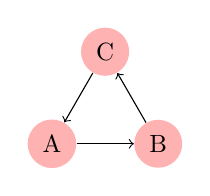
\begin{tikzpicture}[scale=.9, transform shape]
	\tikzstyle{every node} = [circle, fill=red!30]
	\node (a) at (0, 0) {A};
	\node (b) at +(0: 1.5) {B};
	\node (c) at +(60: 1.5) {C};
	\foreach \from / \to in {a/b, b/c, c/a}
		\draw [->] (\from) -- (\to);
\end{tikzpicture}

\end{document}
